\section[Системное описание предметной области и постановка задачи]{%
  СИСТЕМНОЕ ОПИСАНИЕ ПРЕДМЕТНОЙ \\
  ОБЛАСТИ И ПОСТАНОВКА ЗАДАЧИ
}\label{sec:spec}

\subsection{Выбор целевой программной платформы}

Для того, чтобы правильно выбрать платформу, для которой
будет разрабатываться мобильное приложение,
следует сначала оценить состояние и перспективы развития
как рынка мобильных устройств связи в целом, так и конкретных
мобильных платформ в частности.
Под состоянием мобильной платформы здесь понимается доля рынка,
занимаемого данной платформой, а под перспективами развития ---
намерения компании-разработчика и сообщества сторонних разработчиков
эту платформу поддерживать.

В целом, современный рынок мобильных устройств можно охарактеризовать
как <<крупный>> и <<быстро развивающийся>>.
По данным ITU, представленным на рисунке~\ref{fig:stat_phone},
за период с 2005 по 2015 год общее число мобильных устройств в мире увеличилось
более чем в три раза и составило более семи миллиардов~\cite{itu_stat_phone}.

\begin{figure}[h!]
  \centering
  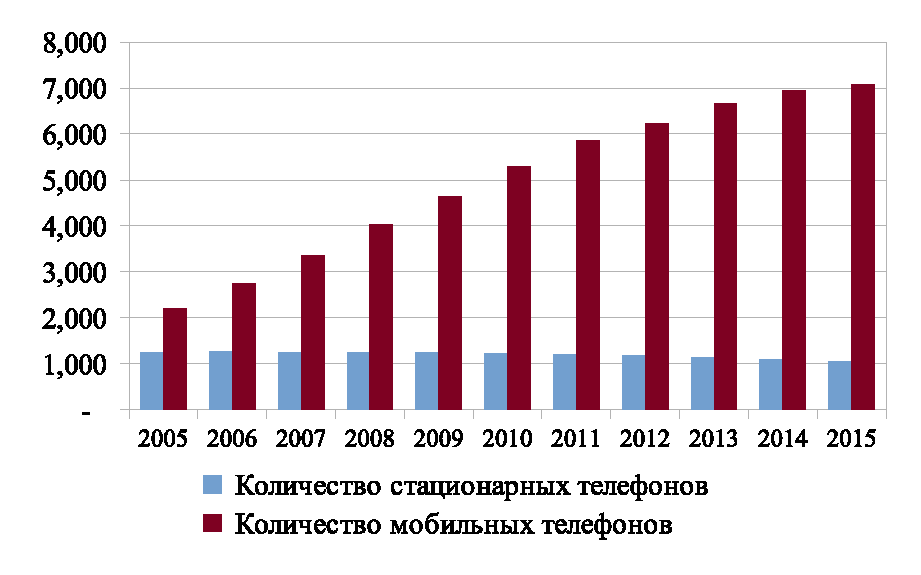
\includegraphics[width=150mm]{fig/stat_phone.eps}
  \caption{Динамика использования персональных устройств связи}
  \label{fig:stat_phone}
\end{figure}

Таким образом, по состоянию на 2015 год, на каждые 100 человек населения земного
шара приходится около 97 мобильных устройств телефонной связи.
Интересно отметить, что общее число станционарных устройств связи
за это время, наоборот, сократилось.

По данным компании Ericsson, в 2015 году было зарегистрировано использование
около 3{,}4 миллиарда смартфонов для доступа в {\color{red} интернет}~\cite{ericsson_mobility_report},
что составляет около 47\% от общего числа мобильных устройств.

Популярность различных мобильных платформ сравнивают, как правило,
по объемам продаж устройств, на которых они предустановлены.
По данным агенства Gartner~\cite{gartner_smartphone_stat}, представленным
в таблице~\ref{tbl:gartner_platform_stat}, можно утверждать, что наиболее популярной
мобильной платформой является Android --- мобильная платформа от
компании Google, занимающая на данный момент около 80\% рынка.

\begin{table} [h!]
  \caption{
    Динамика изменения количества проданных смартфонов под
    управлением различных операционных систем
  }\label{tbl:gartner_platform_stat}
    \begin{tabular}{| m{6.6cm} | c | c | c | c |}
      \hline

      \multirow{2}{*}{
      \parbox{6.6cm}{
      \smallskip
      \centering Операционная система
      \smallskip
      }
      }
      & \multicolumn{2}{c|}{
          \parbox{4.5cm}{
            \smallskip
            \centering Четвертый квартал 2014 года
            \smallskip
          }
        }
      & \multicolumn{2}{c|}{
          \parbox{4.5cm}{
            \smallskip
            \centering Четвертый квартал 2015 года
            \smallskip
          }
        } \\
      \cline{2-5}

      & млн. штук & \% & млн. штук & \% \\
      \hline

      Android &  279 & 76 & 325{,}4 & 80{,}7 \\
      \hline

      iOS &  75 & 20{,}4 & 71{,}5 & 17{,}7 \\
      \hline

      Windows & 10{,}5 & 2{,}8 & 4{,}5 & 1{,}1 \\
      \hline

      Blackberry & 1{,}7 & 0{,}4 & 0{,}9 & 0{,}3 \\
      \hline

      Другие & 1{,}3 & 0{,}4 & 0{,}9 & 0{,}2 \\
      \hline

      Всего & 367{,}5 & 100{,}0 & 400{,}6 & 100{,}0 \\
      \hline
    \end{tabular}
\end{table}

Кроме этого, из приведенных данных видно, что Android является единственной
платформой, доля реализованных мобильных устройств под управлением которой
за наблюдаемый период которой не сократилась.

Android позиционируется как бесплатная платформа для широкого круга устройств
любых производителей, что позволяет снизить конечную стоимость устройства,
что, в свою очередь, обуславливает высокую популярность платформы.
Android имеет открытый исходный код; разработчики ядра платформы
охотно принимают патчи от сторонних разработчиков, поэтому вокруг неё сформировалось
активное сообщество.
Приведенные факты позволяют сделать вывод, что платформа Android является наиболее
перспективной для разработки мобильных приложений.

Весьма актуальным является вопрос выбора минимальной версии Android,
которая должна поддерживаться разрабатываемым мобильным приложением.
Дело в том, что различные версии этой платформы не обладают прямой совместимостью.
Действительно, поддержка только новейших версий Android сужает объем потенциальной
целевой аудитории, а поддержка максимального числа версий значительно усложняет
процесс разработки и тестирования.

На рисунке~\ref{fig:stat_android} представлены официальные
данные об относительной популярности различных версий
ОС Android~\cite{google_stat_android}.

\begin{figure}[h!]
  \centering
  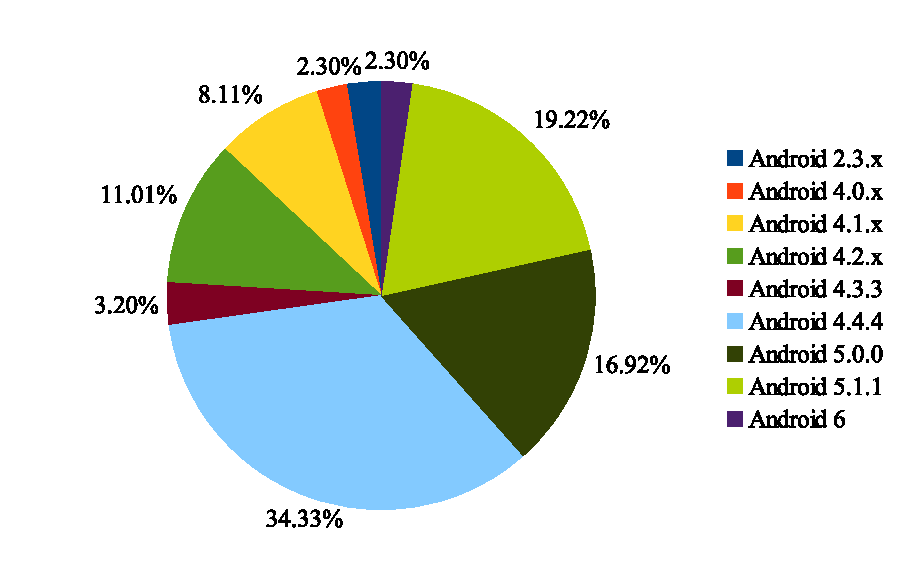
\includegraphics[width=150mm]{fig/stat_android.eps}
  \caption{Относительная популярность различных \\ версий платформы Android}
  \label{fig:stat_android}
\end{figure}

Исходя из этих данных, можно сделать вывод, что наиболее целесообразной
является разработка мобильного приложения для Android версией не ниже 4.0.x.
В этом случае оно будет доступно для 97\% пользователей данной мобильной платформы.


\subsection{Сравнительный анализ существующих приложений-аналогов}

Для более точного определения требований к разрабатываемому приложению
выполним сравнительный анализ существующих приложений.
Сравнительный анализ по опредению предполагает предварительное
описание множества объектов, подвергающихся анализу,
и множества критериев сравнения.
В контексте ОС Android роль рынка приложений выполняет
Google Play Store --- официальный интернет-магазин мобильных приложений,
игр, книг, музыки и видео.

Выполним отбор приложений для анализа следующим образом:
введем типичную поисковую фразу для данной категории приложений,
например, "money manager" и выберем несколько приложений,
расположившихся на верхних позициях выдачи,
для дальнейшего рассмотрения.
Данный подход призван сымитировать поведение типичного пользователя
Play Market, желающего установить себе подобное приложение,
при этом не обладающего какой-либо дополнительной информацией о предмете,
а посему полагающегося на качество поисковых алгоритмов Google.
Данным образом были выбраны следующие приложения, расположенные
в порядке поисковой выдачи:
\begin{itemize}
\item Monefy (автор: MonefyApp);
\item Money Manager Expense \& Budget (Realbyte Inc.);
\item Money Lover --- Money Manager (ZooStudio);
\item Money Manager Ex for Android (Android Money Manager Ex Prj)
\item AndroMoney (AndroMoney);
\item Expense Manager (Bishinews);
\item Money Manager Master (SMH17);
\item Money Manager (Praveen Thogarla).
\end{itemize}

Отметим, что как минимум пять приложений из этого списка поддерживаются
компаниями-разработчиками, что косвенно свидетельствует о сложности данных проектов.
Последний пункт списка на самом деле представляет собой два похожих дргу на друга
одноименных приложения, разработанных индийскими программистами.

Выделим основные категории параметров мобильных приложений, подлежащих сравнению:
\begin{itemize}
\item базовые характеристики;
\item системные характеристики;
\item функциональные возможности;
\item пользовательский интерфейс.
\end{itemize}

Под базовыми характеристиками будем понимать набор параметров приложения,
доступных для оценки без установки приложения. Как правило, эти параметры
создают первое впечатление о приложении у конечного пользователя.
Системные характеристики представляют собой характеристики функционирующего
приложения безотносительно выполняемых им функций.
Набор функциональных возможностей определяет способности приложения
удовлетворять различные запросы пользователя в контексте предметной области.
Пользовательский интерфейс влияет на удобство пользования приложением в целом.

Рассмотрим категорию базовых характеристик приложения.
К числу таких характеристик относятся:
количество загрузок приложения, рейтинг приложения,
стоимость платной версии (если таковая имеется), ограничения бесплатной версии.
Результаты сравнения приложений по данным характеристикам приведены
в таблице~\ref{tbl:cmp_basic}.

\begin{table} [h!]
  \caption{
    Сравнение приложений-аналогов по базовым критериям
  }\label{tbl:cmp_basic}
    \begin{tabular}{| m{4cm} | c | c | c | c | c | c | c | c |}
      \hline
      \parbox{4cm}{
        \smallskip
        \centering Критерий \\ сравнения
        \smallskip
      }
      & \rotatebox[origin=c]{90}{
          \parbox{5cm}{
            Monefy
          }
        }
      & \rotatebox[origin=c]{90}{
          \parbox{5cm}{
            Money Manager \\ Expense \& Budget
          }
        }
      & \rotatebox[origin=c]{90}{
          \parbox{5cm}{
            Money Lover --- \\ Money Manager
          }
        }
      & \rotatebox[origin=c]{90}{
          \parbox{5cm}{
            Andro Money
          }
        }
      & \rotatebox[origin=c]{90}{
          \parbox{5cm}{
            Expense Manager
          }
        }
      & \rotatebox[origin=c]{90}{
          \parbox{5cm}{
            Money Manager Ex \\ for Android
          }
        }
      & \rotatebox[origin=c]{90}{
          \parbox{5cm}{
            Money Manager Master
          }
        }
      & \rotatebox[origin=c]{90}{
          \parbox{5cm}{
            Money Manager
          }
        } \\
      \hline

      Приблизительное \par количество \par загрузок
      & \( 10^6 \)
      & \( 10^6 \)
      & \( 10^6 \)
      & \( 10^6 \)
      & \( 10^6 \)
      & \( 10^5 \)
      & \( 5 \cdot 10^3 \)
      & \( 10^3 \) \\
      \hline

      Рейтинг \par приложения
      & \( 4{,}5 \)
      & \( 4{,}5 \)
      & \( 4{,}5 \)
      & \( 4{,}7 \)
      & \( 4{,}3 \)
      & \( 4{,}4 \)
      & \( 4{,}6 \)
      & \( 4{,}5 \) \\
      \hline

      Ограничения \par бесплатной \par версии
      & Р\tablefootnote{принудительный показ рекламы{\color{red}.}},
        Ф\tablefootnote{ограничения функциональности.}
      & Р, Ф
      & Р, Ф
      & Р
      & Р
      & \( - \)
      & Р, Ф
      & \( - \) \\
      \hline

      Стоимость \par
      платной версии, \$
      & \( 1{,}8 \)
      & \( 3{,}3 \)
      & \( 2{,}2 - 5 \)
      & \( 5 \)
      & \( 5 \)
      & \( - \)
      & \( 2{,}3 - 5 \)
      & \( - \) \\
      \hline
    \end{tabular}
\end{table}

По приведенным данным можно сделать следующие выводы:
\begin{itemize}
  \item данный класс приложений пользуются высоким спросом;
  \item наиболее популярные приложения разрабатываются
    компаниями, а не частными лицами;
  \item монетизация приложений осуществляется в основном за
    счет принудительного показа рекламы в бесплатной версии приложения.
\end{itemize}

К системным характеристикам будем относить
размер установленного приложения и набор прав доступа,
требуемых для его функционирования.
Результат сравнения по этим критериям приведен в таблице~\ref{tbl:cmp_system}.

\begin{table} [h!]
  \caption{
    Сравнение приложений-аналогов по системным критериям
  }\label{tbl:cmp_system}
  \small{
    \begin{tabular}{| m{6.7cm} | c | c | c | c | c | c | c | c |}
      \hline
      \parbox{6.7cm}{
        \smallskip
        \centering Критерий \\ сравнения
        \smallskip
      }
      & \rotatebox[origin=c]{90}{
          \parbox{4.5cm}{
            Monefy
          }
        }
      & \rotatebox[origin=c]{90}{
          \parbox{4.5cm}{
            Money Manager \\ Expense \& Budget
          }
        }
      & \rotatebox[origin=c]{90}{
          \parbox{4.5cm}{
            Money Lover --- \\ Money Manager
          }
        }
      & \rotatebox[origin=c]{90}{
          \parbox{4.5cm}{
            Andro Money
          }
        }
      & \rotatebox[origin=c]{90}{
          \parbox{4.5cm}{
            Expense Manager
          }
        }
      & \rotatebox[origin=c]{90}{
          \parbox{4.5cm}{
            Money Manager Ex \\ for Android
          }
        }
      & \rotatebox[origin=c]{90}{
          \parbox{4.5cm}{
            Money Manager Master
          }
        }
      & \rotatebox[origin=c]{90}{
          \parbox{4.5cm}{
            Money Manager
          }
        } \\
      \hline

      Размер установленного \par приложения, Мб
      & \( 15{,}2 \)
      & \( 12{,}1 \)
      & \( 23{,}4 \)
      & \( 19{,}5 \)
      & \( 7{,}3 \)
      & \( 15{,}8 \)
      & \( 15{,}1 \)
      & \( 1{,}7 \) \\
      \hline

      Запрашиваемые права:
      & & & & & & & & \\

      -- доступ к карте памяти
      & +
      & +
      & +
      & +
      & +
      & +
      & +
      & \\

      -- доступ к сети {\color{red} Интернет}
      & +
      & +
      & +
      & +
      & +
      & +
      & +
      & \\

      -- доступ к Google-аккаунту \par пользователя
      &
      &
      & +
      & +
      & +
      &
      & +
      & \\

      -- управление вибратором
      &
      & +
      & +
      & +
      &
      & +
      &
      & \\

      -- возможность автоматического \par запуска приложения при \par старте системы
      &
      & +
      & +
      & +
      &
      & +
      &
      & \\

      -- возможность предотвращения \par
      автоматического перехода \par
      устройства в энергосберегающий \par
      режим
      &
      & +
      & +
      & +
      &
      &
      &
      & \\

      -- доступ к SMS пользователя
      &
      & +
      &
      & +
      & +
      &
      &
      & \\

      -- доступ к данным GPS
      &
      &
      & +
      &
      &
      &
      & +
      & \\

      -- доступ к телефонному модулю
      &
      & +
      &
      &
      &
      &
      & +
      & \\

      -- доступ к списку активных \par приложений
      &
      & +
      &
      &
      &
      &
      &
      & \\

      -- управление иконками \par рабочего стола
      &
      &
      & +
      &
      &
      &
      &
      & \\

      -- доступ к персональной \par информации\tablefootnote{%
      доступ к событиям календаря, электронной почте и
      прочим персональным данным пользователя.}
      &
      &
      &
      &
      &
      &
      & +
      & \\

      -- доступ к фотокамере
      &
      &
      &
      & +
      &
      &
      &
      & \\
      \hline
    \end{tabular}
  }
\end{table}


Здравый смысл подсказывает, что установленное приложение должно
занимать как можно меньше места и требовать как можно меньше прав доступа.
С другой стороны, с учетом нынешней низкой стоимости ПЗУ,
его объем для современных смартфонов не является критическим ресурсом,
поэтому размер установленного приложения не играет существенной роли.
Иным образом обстоит дело с правами доступа:
с одной стороны, они могут быть необходимы для обеспечения работоспособности
базовых функций приложения
(например, приложение, предоставляющее прогноз погоды, должно иметь доступ в интернет),
использоваться для предоставления дополнительных возможностей
(приложение позволяющее для обмена сообщениями
может потребовать доступ к карте памяти, где хранятся фотографии, для того, чтобы
прикреплять их к основному тексту).
С другой стороны, существует риск, что приложение, написанное недобросовестным
разработчиком, будет использовать предоставленные предоставленные права для достижения
своих целей, (например, рассылать спам или передавать личные данные третьим лицам).

По данным таблицы~\ref{tbl:cmp_system} можно сделать следующие выводы:
\begin{itemize}
\item для работы большинства приложений необходимы досуп к карте памяти и
  {\color{red} сети Интернет};
\item приложения Monefy и Money Manager выгодно отличаются от конкурентов
  минимальным набором прав доступа;
\item некоторые приложения требуют использования прав,
  нетипичных для своего класса.
\end{itemize}

В контексте приведенных выше соображений безопасности, требования приложений
Money Manager Expense \& Budget, Money Lover --- Money Manager,
Andro Money, Expense Manager и Money Manager Master доступа
к пользовательским SMS, данным навигации, телефонному модулю выглядят довольно
подозрительно.
На этом фоне особенно настораживающим является требование приложения
Money Manager Master доступа к персональным данным пользователя.

{\color{red} Введение}

\pagebreak

\begin{table} [h!]
  \caption{
    Функциональные возможности приложений-аналогов
  }\label{tbl:cmp_func}
  \small{
    \begin{tabular}{| m{7.8cm} | c | c | c | c | c | c | c | c |}
      \hline
      \parbox{7.8cm}{
        \smallskip
        \centering \color{red}Функциональные возможности
        \smallskip
      }
      & \rotatebox[origin=c]{90}{
          \parbox{4.5cm}{
            Monefy
          }
        }
      & \rotatebox[origin=c]{90}{
          \parbox{4.5cm}{
            Money Manager \\ Expense \& Budget
          }
        }
      & \rotatebox[origin=c]{90}{
          \parbox{4.5cm}{
            Money Lover --- \\ Money Manager
          }
        }
      & \rotatebox[origin=c]{90}{
          \parbox{4.5cm}{
            Andro Money
          }
        }
      & \rotatebox[origin=c]{90}{
          \parbox{4.5cm}{
            Expense Manager
          }
        }
      & \rotatebox[origin=c]{90}{
          \parbox{4.5cm}{
            Money Manager Ex \\ for Android
          }
        }
      & \rotatebox[origin=c]{90}{
          \parbox{4.5cm}{
            Money Manager Master
          }
        }
      & \rotatebox[origin=c]{90}{
          \parbox{4.5cm}{
            Money Manager
          }
        } \\
      \hline

      Управление данными:
      & & & & & & & & \\

      -- {\color{red} поддержка} нескольких счетов
      & +
      & +
      & +
      & +
      & +
      & +
      & +
      & \\

      -- {\color{red} поддержка} нескольких валют
      &
      & +
      & +
      & +
      & +
      & +
      & +
      & \\

      -- редактирование категорий учета
      & *\tablefootnote{в платной версии.}
      & +
      & +
      & +
      & +
      & +
      & +
      & + \\

      -- поддержка повторяющихся транзакций
      &
      & +
      & +
      & +
      & +
      & +
      & +
      & \\
      \hline

      Представление данных:
      & & & & & & & & \\

      -- группировка данных по времени
      & +
      & +
      & +
      & +
      & +
      & +
      & +
      & + \\

      -- группировка данных по категориям
      & +
      & +
      & +
      & +
      & +
      & +
      & +
      & + \\

      -- группировка данных по типу транзакций
      &
      & +
      & +
      &
      & +
      & +
      & +
      & + \\

      -- представление данных в виде круговых диаграмм
      & +
      & +
      &
      & +
      &
      & +
      & *
      & \\

      -- представление данных в виде {\color{red} графиков}
      &
      & +
      & +
      & +
      & +
      & +
      & *
      & + \\

      \hline

      Дополнительные возможности:
      & & & & & & & & \\

      -- резервное копирование
      & +
      & +
      & +
      & +
      & +
      & +
      &
      & \\

      -- ограничение {\color{red} величины расходов}
      & +
      & +
      & +
      & +
      & +
      & +
      &
      & \\

      -- {\color{red} напоминание} о необходимости ввода данных
      &
      &
      & +
      & +
      &
      &
      &
      & \\

      -- поиск транзакций
      &
      & +
      & +
      & +
      &
      & +
      &
      & \\

      -- парольная защита доступа к данным
      & +
      & +
      &
      & +
      & +
      & +
      &
      & \\

      -- синхронизация данных с удаленным сервером
      & +
      & *
      & +
      & +
      & +
      & +
      &
      & \\

      -- сохранение/загрузка данных из файла
      & +
      & *
      & +
      & +
      & +
      & +
      &
      & \\
      \hline
    \end{tabular}
  }
\end{table}

% Описание проблем, решаемых данным классом мобильных приложений.
% Описание общих требований.
% Формирование критериев оценки существующих приложений.

% Выделение групп приложений со схожими показателями.
% Сравнительный анализ типичных представителей этих групп (не менее 3 представителей).

\subsection{Обзор темы распознавания образов}

Обзор темы распознавания образов.
Этапы процесса распознавания.
Краткое описание алгоримов, используемых на каждом этапе.

Свободное программное обеспечение. Свободные лицензии. Копилефт.

Постановка задачи проектирования.
Уточнение требований к проектируемому приложению. Ввод данных с использованием камеры.